\documentclass[11pt,]{article}
\usepackage[left=0.5in,top=0.75in,right=0.3in,bottom=0.3in]{geometry}
\newcommand*{\authorfont}{\fontfamily{phv}\selectfont}
\usepackage[]{mathpazo}


  \usepackage[T1]{fontenc}
  \usepackage[utf8]{inputenc}



\usepackage{abstract}
\renewcommand{\abstractname}{}    % clear the title
\renewcommand{\absnamepos}{empty} % originally center

\renewenvironment{abstract}
 {{%
    \setlength{\leftmargin}{0mm}
    \setlength{\rightmargin}{\leftmargin}%
  }%
  \relax}
 {\endlist}

\makeatletter
\def\@maketitle{%
  \newpage
%  \null
%  \vskip 2em%
%  \begin{center}%
  \let \footnote \thanks
    {\fontsize{18}{20}\selectfont\raggedright  \setlength{\parindent}{0pt} \@title \par}%
}
%\fi
\makeatother




\setcounter{secnumdepth}{0}

\usepackage{color}
\usepackage{fancyvrb}
\newcommand{\VerbBar}{|}
\newcommand{\VERB}{\Verb[commandchars=\\\{\}]}
\DefineVerbatimEnvironment{Highlighting}{Verbatim}{commandchars=\\\{\}}
% Add ',fontsize=\small' for more characters per line
\usepackage{framed}
\definecolor{shadecolor}{RGB}{248,248,248}
\newenvironment{Shaded}{\begin{snugshade}}{\end{snugshade}}
\newcommand{\AlertTok}[1]{\textcolor[rgb]{0.94,0.16,0.16}{#1}}
\newcommand{\AnnotationTok}[1]{\textcolor[rgb]{0.56,0.35,0.01}{\textbf{\textit{#1}}}}
\newcommand{\AttributeTok}[1]{\textcolor[rgb]{0.77,0.63,0.00}{#1}}
\newcommand{\BaseNTok}[1]{\textcolor[rgb]{0.00,0.00,0.81}{#1}}
\newcommand{\BuiltInTok}[1]{#1}
\newcommand{\CharTok}[1]{\textcolor[rgb]{0.31,0.60,0.02}{#1}}
\newcommand{\CommentTok}[1]{\textcolor[rgb]{0.56,0.35,0.01}{\textit{#1}}}
\newcommand{\CommentVarTok}[1]{\textcolor[rgb]{0.56,0.35,0.01}{\textbf{\textit{#1}}}}
\newcommand{\ConstantTok}[1]{\textcolor[rgb]{0.00,0.00,0.00}{#1}}
\newcommand{\ControlFlowTok}[1]{\textcolor[rgb]{0.13,0.29,0.53}{\textbf{#1}}}
\newcommand{\DataTypeTok}[1]{\textcolor[rgb]{0.13,0.29,0.53}{#1}}
\newcommand{\DecValTok}[1]{\textcolor[rgb]{0.00,0.00,0.81}{#1}}
\newcommand{\DocumentationTok}[1]{\textcolor[rgb]{0.56,0.35,0.01}{\textbf{\textit{#1}}}}
\newcommand{\ErrorTok}[1]{\textcolor[rgb]{0.64,0.00,0.00}{\textbf{#1}}}
\newcommand{\ExtensionTok}[1]{#1}
\newcommand{\FloatTok}[1]{\textcolor[rgb]{0.00,0.00,0.81}{#1}}
\newcommand{\FunctionTok}[1]{\textcolor[rgb]{0.00,0.00,0.00}{#1}}
\newcommand{\ImportTok}[1]{#1}
\newcommand{\InformationTok}[1]{\textcolor[rgb]{0.56,0.35,0.01}{\textbf{\textit{#1}}}}
\newcommand{\KeywordTok}[1]{\textcolor[rgb]{0.13,0.29,0.53}{\textbf{#1}}}
\newcommand{\NormalTok}[1]{#1}
\newcommand{\OperatorTok}[1]{\textcolor[rgb]{0.81,0.36,0.00}{\textbf{#1}}}
\newcommand{\OtherTok}[1]{\textcolor[rgb]{0.56,0.35,0.01}{#1}}
\newcommand{\PreprocessorTok}[1]{\textcolor[rgb]{0.56,0.35,0.01}{\textit{#1}}}
\newcommand{\RegionMarkerTok}[1]{#1}
\newcommand{\SpecialCharTok}[1]{\textcolor[rgb]{0.00,0.00,0.00}{#1}}
\newcommand{\SpecialStringTok}[1]{\textcolor[rgb]{0.31,0.60,0.02}{#1}}
\newcommand{\StringTok}[1]{\textcolor[rgb]{0.31,0.60,0.02}{#1}}
\newcommand{\VariableTok}[1]{\textcolor[rgb]{0.00,0.00,0.00}{#1}}
\newcommand{\VerbatimStringTok}[1]{\textcolor[rgb]{0.31,0.60,0.02}{#1}}
\newcommand{\WarningTok}[1]{\textcolor[rgb]{0.56,0.35,0.01}{\textbf{\textit{#1}}}}

\usepackage{graphicx,grffile}
\makeatletter
\def\maxwidth{\ifdim\Gin@nat@width>\linewidth\linewidth\else\Gin@nat@width\fi}
\def\maxheight{\ifdim\Gin@nat@height>\textheight\textheight\else\Gin@nat@height\fi}
\makeatother
% Scale images if necessary, so that they will not overflow the page
% margins by default, and it is still possible to overwrite the defaults
% using explicit options in \includegraphics[width, height, ...]{}
\setkeys{Gin}{width=\maxwidth,height=\maxheight,keepaspectratio}

\title{Lab 5 Two factor Factorial 1  }



\author{\Large Shen Qu\vspace{0.05in} \newline\normalsize\emph{March 09, 2019}  }


\date{}

\usepackage{titlesec}

\titleformat*{\section}{\normalsize\bfseries}
\titleformat*{\subsection}{\normalsize\itshape}
\titleformat*{\subsubsection}{\normalsize\itshape}
\titleformat*{\paragraph}{\normalsize\itshape}
\titleformat*{\subparagraph}{\normalsize\itshape}


\usepackage{natbib}
\bibliographystyle{plainnat}
\usepackage[strings]{underscore} % protect underscores in most circumstances



\newtheorem{hypothesis}{Hypothesis}
\usepackage{setspace}

\makeatletter
\@ifpackageloaded{hyperref}{}{%
\ifxetex
  \PassOptionsToPackage{hyphens}{url}\usepackage[setpagesize=false, % page size defined by xetex
              unicode=false, % unicode breaks when used with xetex
              xetex]{hyperref}
\else
  \PassOptionsToPackage{hyphens}{url}\usepackage[unicode=true]{hyperref}
\fi
}

\@ifpackageloaded{color}{
    \PassOptionsToPackage{usenames,dvipsnames}{color}
}{%
    \usepackage[usenames,dvipsnames]{color}
}
\makeatother
\hypersetup{breaklinks=true,
            bookmarks=true,
            pdfauthor={Shen Qu (March 09, 2019)},
             pdfkeywords = {},  
            pdftitle={Lab 5 Two factor Factorial 1},
            colorlinks=true,
            citecolor=blue,
            urlcolor=blue,
            linkcolor=magenta,
            pdfborder={0 0 0}}
\urlstyle{same}  % don't use monospace font for urls

% set default figure placement to htbp
\makeatletter
\def\fps@figure{htbp}
\makeatother



% add tightlist ----------
\providecommand{\tightlist}{%
\setlength{\itemsep}{0pt}\setlength{\parskip}{0pt}}

\begin{document}
	
% \pagenumbering{arabic}% resets `page` counter to 1 
%
% \maketitle

{% \usefont{T1}{pnc}{m}{n}
\setlength{\parindent}{0pt}
\thispagestyle{plain}
{\fontsize{18}{20}\selectfont\raggedright 
\maketitle  % title \par  

}

{
   \vskip 13.5pt\relax \normalsize\fontsize{11}{12} 
\textbf{\authorfont Shen Qu} \hskip 15pt \emph{\small March 09, 2019}   

}

}








\begin{abstract}

    \hbox{\vrule height .2pt width 39.14pc}

    \vskip 8.5pt % \small 

\noindent An experiment was designed to study weight gain of rats fed four
different diets, where there were two levels of protein (high or low)
and two sources of protein (beef or cereal). This gives 2 x 2 treatment
combinations: high/beef (HB), high/cereal (HC), low/beef (LB),
low/cereal (LC). Ten rats were in each of the four treatment groups. Use
a=0.01


    \hbox{\vrule height .2pt width 39.14pc}


\end{abstract}


\vskip 6.5pt


\noindent  \begin{enumerate}
\def\labelenumi{(\alph{enumi})}
\tightlist
\item
  Plot the data and report the plot here (A plot with data and means of
  treatment combinations). Do not report code here. Describe the
  observed relationship between two factors.
\end{enumerate}

\begin{verbatim}
## Observations: 40
## Variables: 5
## $ Source <chr> "Beef", "Beef", "Beef", "Beef", "Beef", "Beef", "Beef",...
## $ Amount <chr> "Low", "Low", "Low", "Low", "Low", "Low", "Low", "Low",...
## $ Gain   <dbl> 90, 76, 90, 64, 86, 51, 72, 90, 95, 78, 73, 102, 118, 1...
## $ Trt1   <fct> Beef, Beef, Beef, Beef, Beef, Beef, Beef, Beef, Beef, B...
## $ Trt2   <fct> Low, Low, Low, Low, Low, Low, Low, Low, Low, Low, High,...
\end{verbatim}

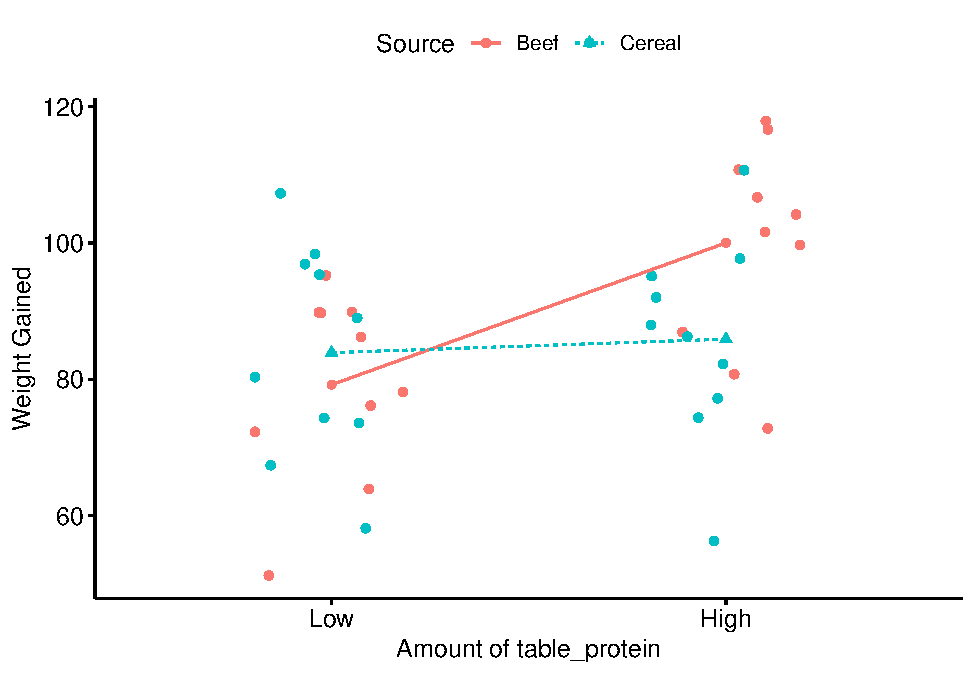
\includegraphics[width=0.5\linewidth]{svm-rmarkdown-article-example_files/figure-latex/unnamed-chunk-3-1}

\begin{enumerate}
\def\labelenumi{(\alph{enumi})}
\setcounter{enumi}{1}
\tightlist
\item
  Obtain the numerical summary for each treatment combination and factor
  levels separately. Report them here in a tabular form.
\end{enumerate}

\begin{verbatim}
##   Source min   Q1 median    Q3 max mean       sd  n missing
## 1   Beef  51 77.5     90 102.5 118 89.6 17.71232 20       0
## 2 Cereal  56 74.0     87  95.5 111 84.9 14.99438 20       0
\end{verbatim}

\begin{verbatim}
##   Amount min    Q1 median     Q3 max  mean       sd  n missing
## 1   High  56 81.75   93.5 104.75 118 92.95 16.36259 20       0
## 2    Low  51 73.50   83.0  91.25 107 81.55 14.63045 20       0
\end{verbatim}

\begin{verbatim}
##        Amount min    Q1 median     Q3 max   mean       sd  n missing
## 1   Beef.High  73 90.25  103.0 110.00 118 100.00 15.13642 10       0
## 2 Cereal.High  56 78.25   87.0  94.25 111  85.90 15.02184 10       0
## 3    Beef.Low  51 73.00   82.0  90.00  95  79.20 13.88684 10       0
## 4  Cereal.Low  58 74.00   84.5  96.50 107  83.90 15.70881 10       0
## 5        High  56 81.75   93.5 104.75 118  92.95 16.36259 20       0
## 6         Low  51 73.50   83.0  91.25 107  81.55 14.63045 20       0
\end{verbatim}

\begin{enumerate}
\def\labelenumi{(\alph{enumi})}
\setcounter{enumi}{2}
\tightlist
\item
  Fit the two-factor factorial model and report the complete ANOVA table
  here. Do not report code here. The complete ANOVA table should have a
  row for each of the following: main effects of each treatment,
  two-factor interaction effects, error and total.
\end{enumerate}

\begin{verbatim}
##             Df Sum Sq Mean Sq F value Pr(>F)  
## Trt1         1    221   220.9   0.988 0.3269  
## Trt2         1   1300  1299.6   5.812 0.0211 *
## Trt1:Trt2    1    884   883.6   3.952 0.0545 .
## Residuals   36   8049   223.6                 
## ---
## Signif. codes:  0 '***' 0.001 '**' 0.01 '*' 0.05 '.' 0.1 ' ' 1
\end{verbatim}

\begin{enumerate}
\def\labelenumi{(\alph{enumi})}
\setcounter{enumi}{3}
\tightlist
\item
  Based on the ANOVA table write your conclusion appropriately. Perform
  all the necessary tests and report the conclusion along with the
  p-value.
\end{enumerate}

\begin{Shaded}
\begin{Highlighting}[]
\KeywordTok{pairwise.t.test}\NormalTok{(table_protein}\OperatorTok{$}\NormalTok{Gain, table_protein}\OperatorTok{$}\NormalTok{Trt2, }\DataTypeTok{p.adj =} \StringTok{"none"}\NormalTok{)}
\end{Highlighting}
\end{Shaded}

\begin{verbatim}
## 
##  Pairwise comparisons using t tests with pooled SD 
## 
## data:  table_protein$Gain and table_protein$Trt2 
## 
##     High 
## Low 0.026
## 
## P value adjustment method: none
\end{verbatim}

\begin{Shaded}
\begin{Highlighting}[]
\KeywordTok{pairwise.t.test}\NormalTok{(table_protein}\OperatorTok{$}\NormalTok{Gain, table_protein}\OperatorTok{$}\NormalTok{Trt2, }\DataTypeTok{p.adj =} \StringTok{"bonf"}\NormalTok{)}
\end{Highlighting}
\end{Shaded}

\begin{verbatim}
## 
##  Pairwise comparisons using t tests with pooled SD 
## 
## data:  table_protein$Gain and table_protein$Trt2 
## 
##     High 
## Low 0.026
## 
## P value adjustment method: bonferroni
\end{verbatim}

\begin{Shaded}
\begin{Highlighting}[]
\KeywordTok{plot}\NormalTok{(}\KeywordTok{LSD.test}\NormalTok{(model_protein, }\DataTypeTok{trt =} \StringTok{"Trt2"}\NormalTok{, }\DataTypeTok{alpha =} \FloatTok{0.05}\NormalTok{))}
\end{Highlighting}
\end{Shaded}

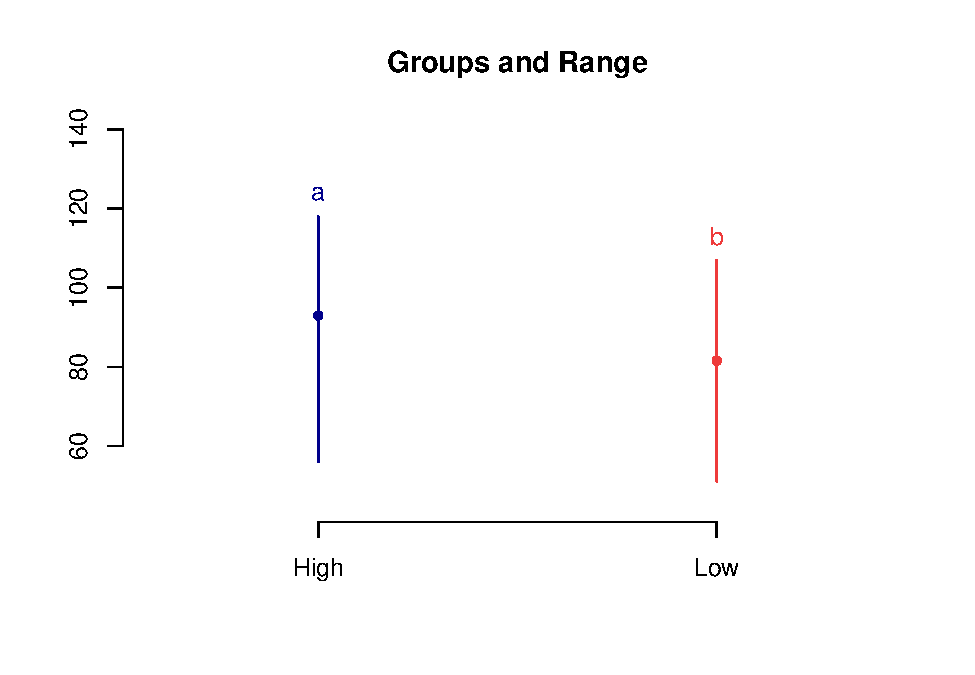
\includegraphics{svm-rmarkdown-article-example_files/figure-latex/unnamed-chunk-6-1.pdf}

\begin{Shaded}
\begin{Highlighting}[]
\NormalTok{(}\KeywordTok{LSD.test}\NormalTok{(model_protein, }\DataTypeTok{trt =} \StringTok{"Trt2"}\NormalTok{, }\DataTypeTok{alpha =} \FloatTok{0.05}\NormalTok{))}
\end{Highlighting}
\end{Shaded}

\begin{verbatim}
## $statistics
##    MSerror Df  Mean       CV  t.value  LSD
##   223.5944 36 87.25 17.13819 2.028094 9.59
## 
## $parameters
##         test p.ajusted name.t ntr alpha
##   Fisher-LSD      none   Trt2   2  0.05
## 
## $means
##       Gain      std  r      LCL      UCL Min Max   Q25  Q50    Q75
## High 92.95 16.36259 20 86.16885 99.73115  56 118 81.75 93.5 104.75
## Low  81.55 14.63045 20 74.76885 88.33115  51 107 73.50 83.0  91.25
## 
## $comparison
## NULL
## 
## $groups
##       Gain groups
## High 92.95      a
## Low  81.55      b
## 
## attr(,"class")
## [1] "group"
\end{verbatim}

\begin{Shaded}
\begin{Highlighting}[]
\KeywordTok{TukeyHSD}\NormalTok{(model_protein, }\DataTypeTok{conf.level =} \FloatTok{0.95}\NormalTok{)}
\end{Highlighting}
\end{Shaded}

\begin{verbatim}
##   Tukey multiple comparisons of means
##     95% family-wise confidence level
## 
## Fit: aov(formula = Gain ~ Trt1 * Trt2, data = table_protein)
## 
## $Trt1
##             diff    lwr  upr     p adj
## Cereal-Beef -4.7 -14.29 4.89 0.3268783
## 
## $Trt2
##           diff    lwr   upr     p adj
## Low-High -11.4 -20.99 -1.81 0.0211449
## 
## $`Trt1:Trt2`
##                         diff      lwr       upr     p adj
## Cereal:High-Beef:High  -14.1 -32.1102  3.910198 0.1697711
## Beef:Low-Beef:High     -20.8 -38.8102 -2.789802 0.0182745
## Cereal:Low-Beef:High   -16.1 -34.1102  1.910198 0.0936982
## Beef:Low-Cereal:High    -6.7 -24.7102 11.310198 0.7492577
## Cereal:Low-Cereal:High  -2.0 -20.0102 16.010198 0.9905411
## Cereal:Low-Beef:Low      4.7 -13.3102 22.710198 0.8952934
\end{verbatim}

\begin{Shaded}
\begin{Highlighting}[]
\KeywordTok{ScheffeTest}\NormalTok{(model_protein, }\DataTypeTok{conf.level =} \FloatTok{0.95}\NormalTok{)}
\end{Highlighting}
\end{Shaded}

\begin{verbatim}
## 
##   Posthoc multiple comparisons of means : Scheffe Test 
##     95% family-wise confidence level
## 
## $Trt1
##             diff    lwr.ci   upr.ci   pval    
## Cereal-Beef -4.7 -18.56594 9.165941 0.8042    
## 
## $Trt2
##           diff    lwr.ci   upr.ci   pval    
## Low-High -11.4 -25.26594 2.465941 0.1410    
## 
## $`Trt1:Trt2`
##                         diff   lwr.ci    upr.ci   pval    
## Cereal:High-Beef:High  -14.1 -33.7094  5.509402 0.2358    
## Beef:Low-Beef:High     -20.8 -40.4094 -1.190598 0.0338 *  
## Cereal:Low-Beef:High   -16.1 -35.7094  3.509402 0.1418    
## Beef:Low-Cereal:High    -6.7 -26.3094 12.909402 0.8004    
## Cereal:Low-Cereal:High  -2.0 -21.6094 17.609402 0.9929    
## Cereal:Low-Beef:Low      4.7 -14.9094 24.309402 0.9195    
## 
## ---
## Signif. codes:  0 '***' 0.001 '**' 0.01 '*' 0.05 '.' 0.1 ' ' 1
\end{verbatim}

\begin{enumerate}
\def\labelenumi{(\alph{enumi})}
\setcounter{enumi}{4}
\tightlist
\item
  Provide the plots of residuals here. Do not report code here.
\end{enumerate}

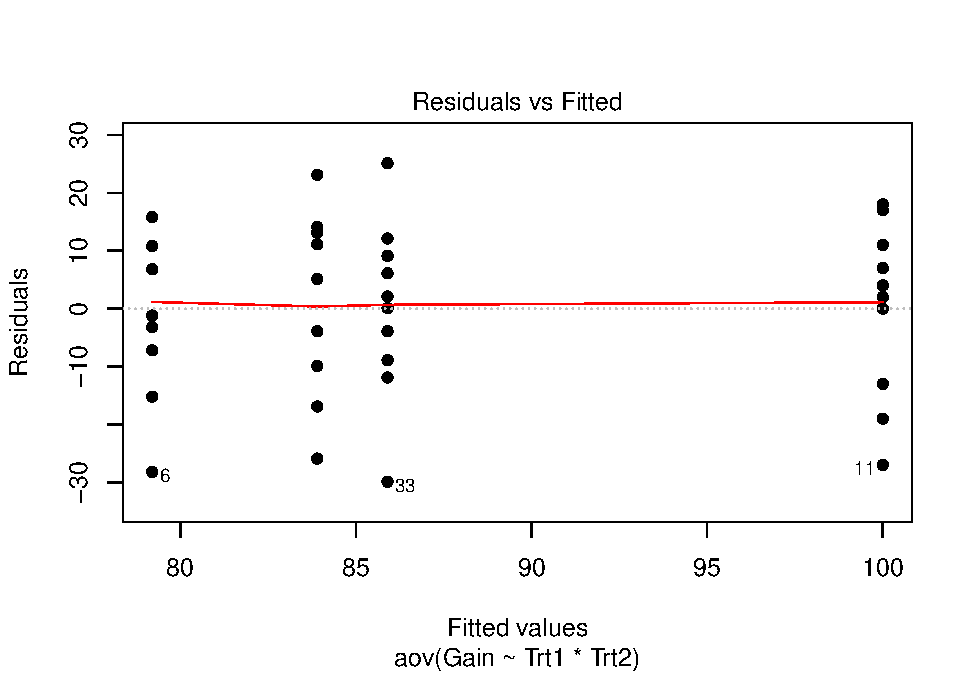
\includegraphics[width=0.25\linewidth]{svm-rmarkdown-article-example_files/figure-latex/unnamed-chunk-7-1}
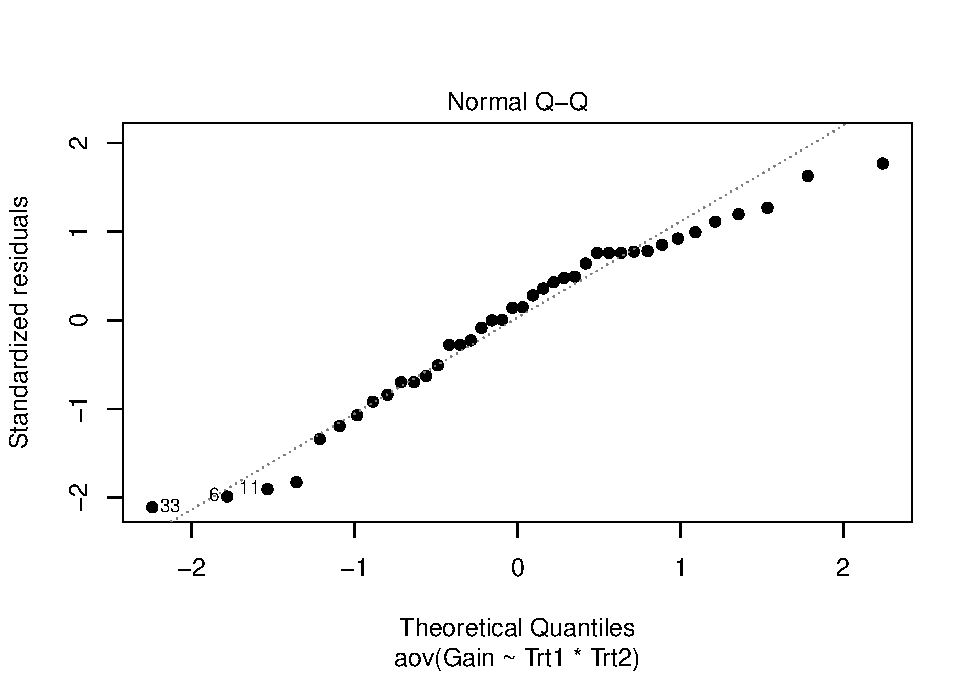
\includegraphics[width=0.25\linewidth]{svm-rmarkdown-article-example_files/figure-latex/unnamed-chunk-7-2}
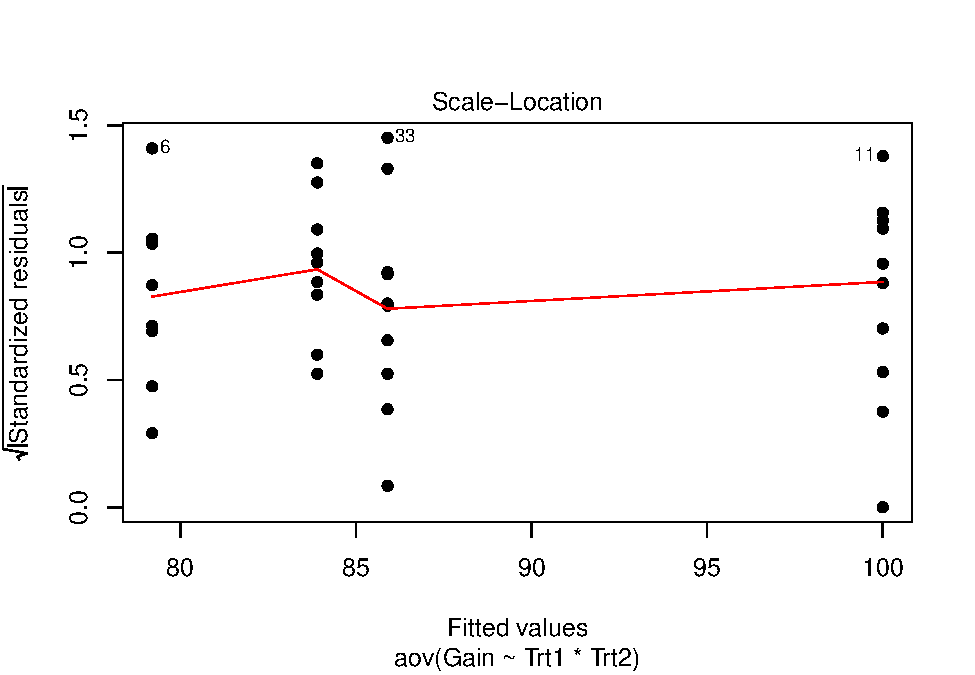
\includegraphics[width=0.25\linewidth]{svm-rmarkdown-article-example_files/figure-latex/unnamed-chunk-7-3}
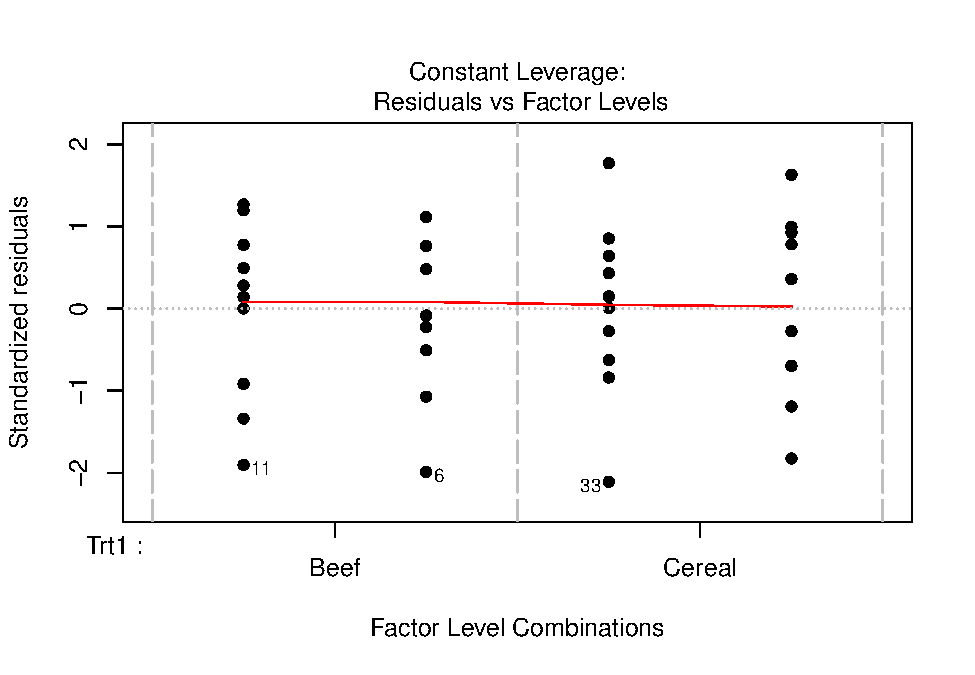
\includegraphics[width=0.25\linewidth]{svm-rmarkdown-article-example_files/figure-latex/unnamed-chunk-7-4}

\begin{enumerate}
\def\labelenumi{(\alph{enumi})}
\setcounter{enumi}{5}
\item
  Based on the residual plots, clearly explain whether assumptions in
  the model are satisfied or violated.
\item
  Report the code here without output.
\end{enumerate}

\begin{Shaded}
\begin{Highlighting}[]
\NormalTok{table_protein <-}\StringTok{ }\KeywordTok{read_excel}\NormalTok{(}\StringTok{"Protein.xlsx"}\NormalTok{)}
\KeywordTok{glimpse}\NormalTok{(table_protein)}

\CommentTok{# Install and load ggplot2 package before using ggplot function #}
\KeywordTok{ggplot}\NormalTok{(}\DataTypeTok{data =}\NormalTok{ table_protein, }\KeywordTok{aes}\NormalTok{(}\DataTypeTok{x =}\NormalTok{ Amount, }\DataTypeTok{y =}\NormalTok{ Gain, }\DataTypeTok{colour =}\NormalTok{ Source, }\DataTypeTok{group =}\NormalTok{ Source)) }\OperatorTok{+}\StringTok{ }
\StringTok{    }\KeywordTok{geom_point}\NormalTok{(}\KeywordTok{aes}\NormalTok{(}\DataTypeTok{shape =}\NormalTok{ Source, }\DataTypeTok{color =}\NormalTok{ Source), }\DataTypeTok{size =} \DecValTok{2}\NormalTok{) }\OperatorTok{+}\StringTok{ }\KeywordTok{labs}\NormalTok{(}\DataTypeTok{y =} \StringTok{"Weight Gained"}\NormalTok{, }
    \DataTypeTok{x =} \StringTok{"Amount of table_protein"}\NormalTok{, }\DataTypeTok{color =} \StringTok{"Source of table_protein"}\NormalTok{, }\DataTypeTok{shape =} \StringTok{"Source of table_protein"}\NormalTok{)}

\CommentTok{# Plots the Mean and 1SD error bars for each treatment group #}
\KeywordTok{ggplot}\NormalTok{(}\DataTypeTok{data =}\NormalTok{ table_protein, }\KeywordTok{aes}\NormalTok{(}\DataTypeTok{x =}\NormalTok{ Amount, }\DataTypeTok{y =}\NormalTok{ Gain, }\DataTypeTok{colour =}\NormalTok{ Source, }\DataTypeTok{shape =}\NormalTok{ Source, }
    \DataTypeTok{group =}\NormalTok{ Source)) }\OperatorTok{+}\StringTok{ }\KeywordTok{stat_summary}\NormalTok{() }\OperatorTok{+}\StringTok{ }\KeywordTok{labs}\NormalTok{(}\DataTypeTok{y =} \StringTok{"Weight Gained"}\NormalTok{, }\DataTypeTok{x =} \StringTok{"Amount of table_protein"}\NormalTok{, }
    \DataTypeTok{color =} \StringTok{"Source"}\NormalTok{, }\DataTypeTok{shape =} \StringTok{"Source"}\NormalTok{)}

\CommentTok{# Install and load ggpubr package before using ggline function #}
\KeywordTok{ggline}\NormalTok{(}\DataTypeTok{data =}\NormalTok{ table_protein, }\DataTypeTok{x =} \StringTok{"Amount"}\NormalTok{, }\DataTypeTok{y =} \StringTok{"Gain"}\NormalTok{, }\DataTypeTok{add =} \KeywordTok{c}\NormalTok{(}\StringTok{"mean"}\NormalTok{, }\StringTok{"jitter"}\NormalTok{), }
    \DataTypeTok{shape =} \StringTok{"Source"}\NormalTok{, }\DataTypeTok{color =} \StringTok{"Source"}\NormalTok{, }\DataTypeTok{linetype =} \StringTok{"Source"}\NormalTok{, }\DataTypeTok{ylab =} \StringTok{"Weight Gained"}\NormalTok{, }
    \DataTypeTok{xlab =} \StringTok{"Amount of table_protein"}\NormalTok{)}

\CommentTok{# Load mosaic package before using favstats function#}
\KeywordTok{favstats}\NormalTok{(Gain }\OperatorTok{~}\StringTok{ }\NormalTok{Source, }\DataTypeTok{data =}\NormalTok{ table_protein)}
\KeywordTok{favstats}\NormalTok{(Gain }\OperatorTok{~}\StringTok{ }\NormalTok{Amount, }\DataTypeTok{data =}\NormalTok{ table_protein)}
\KeywordTok{favstats}\NormalTok{(Gain }\OperatorTok{~}\StringTok{ }\NormalTok{Source }\OperatorTok{|}\StringTok{ }\NormalTok{Amount, }\DataTypeTok{data =}\NormalTok{ table_protein)}
\CommentTok{# favstats(Gain ~ Source+Amount, data=table_protein)}

\CommentTok{# Create Categorical variables so that plot of residuals versus each}
\CommentTok{# treatment combination can be obtained using plot function with the fitted}
\CommentTok{# model later #}
\NormalTok{table_protein}\OperatorTok{$}\NormalTok{Trt1 =}\StringTok{ }\KeywordTok{as.factor}\NormalTok{(table_protein}\OperatorTok{$}\NormalTok{Source)}
\NormalTok{table_protein}\OperatorTok{$}\NormalTok{Trt2 =}\StringTok{ }\KeywordTok{as.factor}\NormalTok{(table_protein}\OperatorTok{$}\NormalTok{Amount)}

\NormalTok{model_protein <-}\StringTok{ }\KeywordTok{aov}\NormalTok{(Gain }\OperatorTok{~}\StringTok{ }\NormalTok{Trt1 }\OperatorTok{*}\StringTok{ }\NormalTok{Trt2, }\DataTypeTok{data =}\NormalTok{ table_protein)}
\KeywordTok{summary}\NormalTok{(model_protein)}
\KeywordTok{plot}\NormalTok{(model_protein, }\DataTypeTok{pch =} \DecValTok{16}\NormalTok{)}

\CommentTok{# Pairwise comparisons using t tests with pooled Standard Deviation # The}
\CommentTok{# output gives a matrix of p values for each pair of treatments #}
\KeywordTok{pairwise.t.test}\NormalTok{(table_protein}\OperatorTok{$}\NormalTok{Gain, table_protein}\OperatorTok{$}\NormalTok{Trt2, }\DataTypeTok{p.adj =} \StringTok{"none"}\NormalTok{)}

\CommentTok{# Pairwise comparisons using t tests with pooled Standard Deviation and}
\CommentTok{# Bonferroni adjustment # The output gives a matrix of p values for each}
\CommentTok{# pair of treatments #}
\KeywordTok{pairwise.t.test}\NormalTok{(table_protein}\OperatorTok{$}\NormalTok{Gain, table_protein}\OperatorTok{$}\NormalTok{Trt2, }\DataTypeTok{p.adj =} \StringTok{"bonf"}\NormalTok{)}

\CommentTok{# Install and load the agricolae package before running the LSD.test}
\CommentTok{# function below # p.adj option in the LSD.test function can be used to}
\CommentTok{# apply different adjustments to control error rates#}
\KeywordTok{plot}\NormalTok{(}\KeywordTok{LSD.test}\NormalTok{(model_protein, }\DataTypeTok{trt =} \StringTok{"Trt2"}\NormalTok{, }\DataTypeTok{alpha =} \FloatTok{0.05}\NormalTok{))}
\CommentTok{# The treatments sharing the same letter on the plot are not different#}

\NormalTok{(}\KeywordTok{LSD.test}\NormalTok{(model_protein, }\DataTypeTok{trt =} \StringTok{"Trt2"}\NormalTok{, }\DataTypeTok{alpha =} \FloatTok{0.05}\NormalTok{))  }\CommentTok{# Using outer parentheses prints the output#}

\CommentTok{# Tukey's test to get observed difference in means, CI and p value#}
\KeywordTok{TukeyHSD}\NormalTok{(model_protein, }\DataTypeTok{conf.level =} \FloatTok{0.95}\NormalTok{)}

\CommentTok{# Scheffe's test to get observed difference in means, CI and p value #}
\CommentTok{# Install and load the DescTools package before using the ScheffeTest}
\CommentTok{# function #}
\KeywordTok{ScheffeTest}\NormalTok{(model_protein, }\DataTypeTok{conf.level =} \FloatTok{0.95}\NormalTok{)}
\end{Highlighting}
\end{Shaded}




\newpage
\singlespacing 
\end{document}
